% Beamer presentation
\documentclass[11pt,aspectratio=43,ignorenonframetext,t]{beamer}

% Presentation settings
\mode<presentation>{
  \usetheme[framenumber,titleframestart=1]{UoM_alex}
  \usefonttheme{professionalfonts} % using non standard fonts for beamer
  \usefonttheme{serif}
  \usepackage{fontspec}
  \setmainfont[Ligatures=TeX]{Arial}
}

% Handout settings
\mode<article>{
  \usepackage{fullpage}
  \usepackage{fontspec}
  \setmainfont[Ligatures=TeX]{Arial}
  \setlength{\parskip}{1.5\baselineskip} % correct beamer line spacings
  \setlength{\parindent}{0cm}
  \usepackage{enumitem}
  \setlist[itemize]{topsep=0pt}
}

 % Packages
\usepackage{graphicx}
\graphicspath{{./images/png}} % generic graphics path; overridden if necessary
\usepackage{amsmath}
\allowdisplaybreaks[1] % allow eqnarrays to break across pages
\usepackage{amssymb} 
\usepackage[HTML]{xcolor}
\definecolor{uomlinkblue}{HTML}{0071BC}
\usepackage{hyperref}
\hypersetup{
  colorlinks=true,
  linkcolor=uomlinkblue,
  filecolor=uomlinkblue,      
  urlcolor=uomlinkblue,
  pdflang={en-GB},
}
\usepackage[document]{ragged2e} % left aligned text for accessibility
\usepackage{tikz}
\usetikzlibrary{positioning, arrows, arrows.meta}
\usepackage{unicode-math} % unicode maths for accessibility
\usepackage{pdfcomment}   % for alt text for accessibility
\usepackage{rotating}     % allow portrait figures and tables
\usepackage{subfigure}    % allow matrices of figures
\usepackage{float}        % allows H option on floats to force here placement
\usepackage{multirow}     % allows merging of rows in tables
\usepackage{tabularx}     % allows fixed width tables
\usepackage{ctable}       % modifies \hline for use in table
\usepackage{bm}           % allow bold fonts in equations
\usepackage{pgf}          % allow graphics manipulation
\usepackage{etoolbox}
  
% Custom commands
\newcolumntype{Z}{>{\centering\arraybackslash}X}  % tabularx centered columns 

\makeatletter
  \DeclareRobustCommand{\em}
  {
    \@nomath\em
    \if b
      \expandafter\@car\f@series\@nil \normalfont
    \else
      \bfseries
    \fi
  }
\makeatother

\makeatletter
  \preto{\@verbatim}{\topsep=0pt \partopsep=0pt}
\makeatother

\def\checkmark{
  \tikz\fill[scale=0.4](0,.35) -- (.25,0) -- (1,.7) -- (.25,.15) -- cycle;
}

% Counters
\newcounter{example_number} % keep track of the example questions

% Frontmatter
\newcommand{\cmclecture}[1]{
  \title{Combinatorial Mesh Calculus (CMC): Lecture #1}
}
\author{
  Lectured by:
  \href{https://scholar.google.com/citations?user=x4R-snQAAAAJ&hl=en}
  {Dr. Kiprian Berbatov}$^1$\\
  \smallskip
  Lecture Notes Compiled by:
  \href{https://scholar.google.com/citations?user=CoIpITkAAAAJ&hl=en}
  {Muhammad Azeem}$^1$\\
  \smallskip
  Under the supervision of:
  \href{https://scholar.google.co.uk/citations?user=3nWJe5wAAAAJ&hl=en}
  {Prof. Andrey P. Jivkov}$^1$\\
  \smallskip
  {\tiny $^1$Department of Mechanical and Aerospace Engineering,
    The University of Manchester, Oxford Road, Manchester M13 9PL, UK}
}

% Special frames
\newcommand{\cmctitleframe}{
  \titlepage
  \begin{tikzpicture}[remember picture,overlay]
    \node[anchor=south east] at (current page.south east) {
      \href{https://youtube.com/@kipi.berbatov}{
        \includegraphics[width=1.5cm]{youtube-icon.png}
      }
    };
  \end{tikzpicture}
}
\newcommand{\cmcendframe}{
  \begin{figure}
    \centering
    \includegraphics[width=0.85\linewidth]{Thanks.png}
  \end{figure}
}

\cmclecture{13}
\date{03 November 2025}

\begin{document}

%========================= TITLE =========================
\begin{frame}
  \cmctitleframe
\end{frame}

\begin{frame}{Integration on Manifolds}
\begin{block}{Definition}
Let $(M,g)$ be a compact oriented $D$–dimensional Riemannian manifold.
\begin{enumerate}
\item The \textbf{measure} of $M$ (length, area, or volume for $D=1,2,3$) is
\begin{align*}
\mu(M)=\int_M \mathrm{vol}_{(M,g)} > 0.
\end{align*}
\item The \textbf{Riemann integral} of a smooth function $f\in\mathcal{F}(M)$ is
\begin{align*}
I(f)=\int_M f\,\mathrm{vol}_{(M,g)}.
\end{align*}
\end{enumerate}
\end{block}
\end{frame}


\begin{frame}{Integration on Manifolds}
\begin{block}{Definition}
For $D=1$, $M=[a,b]$, this reduces to the classical integral
\begin{align*}
I(f)=\int_a^b f(x)\,dx.
\end{align*}
\begin{enumerate}
\item[3] The \textbf{inner product} of two $p$–forms $\omega,\eta\in\Omega^p(M)$ with $p\in\{ 0,1,\dots,D\}$, is
\begin{align*}
\langle \omega,\eta\rangle_p :=& I(g_p(\omega,\eta)).\\
 =& \int_M g_p^*(\omega,\eta)\,\mathrm{vol}_{(M,g)}.
\end{align*}
\end{enumerate}
\end{block}
\end{frame}

% ----------------------------------------------------------
\begin{frame}{Example: Area on the Sphere $S^2_r$}
\begin{block}{Setup}
Let $D=2$, $M=S^2_r=\{(x,y,z)\in\mathbb{R}^3 \mid x^2+y^2+z^2=r^2\}$
with the induced orientation and metric from $\mathbb{R}^3$.
In spherical coordinates:
\begin{align*}
x &= r\sin\theta\cos\phi, &
y &= r\sin\theta\sin\phi, &
z &= r\cos\theta,\\
\theta &\in(0,\pi), &
\phi &\in(0,2\pi).
\end{align*}
The induced metric is $g=r^2(d\theta^2+\sin^2\theta\,d\phi^2)$,
and the volume form is
\begin{align*}
\mathrm{vol}_{(M,g)}=r^2\sin\theta\,d\theta\wedge d\phi.
\end{align*}
\end{block}

\end{frame}

\begin{frame}{Example}
    \begin{block}{Computation of Area of a Spherical Quadrilateral}
For $\theta\in[\theta_1,\theta_2]$ and $\phi\in[\phi_1,\phi_2]$,
\begin{align*}
A &= \int_{[\theta_1,\theta_2]\times[\phi_1,\phi_2]} r^2\sin\theta\,d\theta\wedge d\phi\\
  &= r^2\int_{\phi_1}^{\phi_2}\!\!\int_{\theta_1}^{\theta_2}\sin\theta\,d\theta\,d\phi\\
  &= r^2(\phi_2-\phi_1)(\cos\theta_1-\cos\theta_2).
\end{align*}
This agrees with the Frobenius theorem, ensuring the integration of a $2$–form depends only on the orientation of $M$.
\end{block}
\end{frame}


\begin{frame}{Visualization}
    \begin{block}{}
        \begin{center}
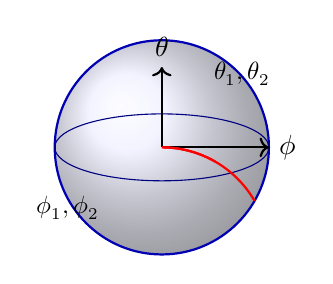
\begin{tikzpicture}[scale=0.85]
\shade[ball color=blue!10,opacity=0.6] (0,0) circle (1.6);
\draw[blue!70!black,thick] (0,0) circle (1.6);
\draw[blue!50!black] (0,0) ellipse (1.6 and 0.5);
\draw[->,thick] (0,0)--(1.6,0) node[right]{$\phi$};
\draw[->,thick] (0,0)--(0,1.2) node[above]{$\theta$};
\draw[red,thick] (0,0) arc (90:60:1.6);
\draw[red,thick] (0,0) arc (90:30:1.6);
\node at (1.2,1.1) {\small $\theta_1,\theta_2$};
\node at (-1.4,-0.9) {\small $\phi_1,\phi_2$};
\end{tikzpicture}
\end{center}
    \end{block}
\end{frame}


% ----------------------------------------------------------
\begin{frame}{Codifferential Operator Manifolds}
\begin{block}{Definition}
Let $(M,g)$ be a compact oriented $D$–dimensional Riemannian manifold, and $p\in\{1,2,\dots,D\}$.
Denote by $\overset{\circ}{\Omega}^p(M)=\{\omega\in\Omega^p(M)\mid \operatorname{tr}_{\partial M}\omega=0\}$
the space of $p$–forms vanishing on the boundary.

The \textbf{codifferential}
\begin{align*}
d_p^*:\overset{\circ}{\Omega}^p(M)\longrightarrow \overset{\circ}{\Omega}^{p-1}(M)
\end{align*}
is the adjoint of $d_{p-1}$ restricted to $\overset{\circ}{\Omega}^{p-1}(M)$:
\begin{align*}
\langle d_p^*\omega,\eta\rangle_{p-1}
=\langle \omega,d_{p-1}\eta\rangle_p,
\qquad
\forall \omega\in \overset{\circ}{\Omega}^p(M),\ \eta\in \overset{\circ}{\Omega}^{p-1}(M).
\end{align*}
\end{block}
\end{frame}

% ----------------------------------------------------------
\begin{frame}{Expression via Hodge Star}
\vspace{-0.2cm}
\begin{block}{Equivalent Expression}
For any $p\in\{1,\dots,D\}$,
\begin{align*}
d_{D-p}^* \circ \star_p
&= (-1)^{p+1}\,\star_{p+1}\circ d_p,\\
\text{or equivalently:}\quad
d_{D-p}^*
&= (-1)^{p+1}\,\star_{p+1}\circ d_p\circ \star_p^{-1}\\
=& (-1)^{p+1+p(D-p)}\,\star_{p+1}\circ d_p\circ \star_{D-p}.
\end{align*}
\end{block}

\vspace{-0.2cm}
\begin{center}
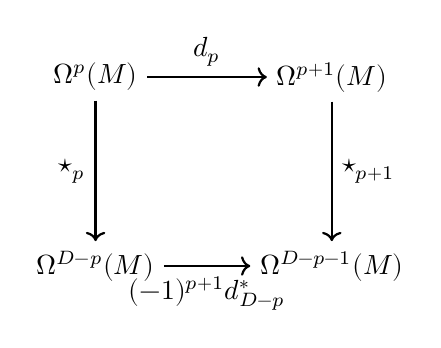
\begin{tikzpicture}[scale=1.0]
\node (a) at (0,1.2) {$\Omega^p(M)$};
\node (b) at (3,1.2) {$\Omega^{p+1}(M)$};
\node (c) at (0,-1.2) {$\Omega^{D-p}(M)$};
\node (d) at (3,-1.2) {$\Omega^{D-p-1}(M)$};

\draw[->,thick] (a)--(b) node[midway,above]{$d_p$};
\draw[->,thick] (a)--(c) node[midway,left]{$\star_p$};
\draw[->,thick] (b)--(d) node[midway,right]{$\star_{p+1}$};
\draw[->,thick] (c)--(d) node[midway,below]{$(-1)^{p+1}d_{D-p}^*$};
\end{tikzpicture}
\end{center}
\end{frame}



\begin{frame}{Codifferential: General Identity}
\begin{block}{Setup and Symbols}
\vspace{-0.7cm}
\begin{align*}
&\text{$(M,g)$: oriented $D$-dimensional Riemannian manifold.}\\
&\Omega^p(M): \text{$p$-forms on $M$},\\
&d_p:\Omega^p(M)\to\Omega^{p+1}(M).\\
&\star_p:\Omega^p(M)\to\Omega^{D-p}(M)\ \text{(Hodge star)},\\
&\star_p^{-1}=(-1)^{p(D-p)}\,\star_{D-p}.\\
&\text{Inner product: } g_p^*(\omega,\eta)\, \mathrm{vol}_g=\omega\wedge\star_p\eta,\\
&\langle \omega,\eta\rangle_p=\int_M g_p^*(\omega,\eta)\,\mathrm{vol}_g.
\end{align*}
\end{block}
\end{frame}

\begin{frame}{Adjoint of $d$}
    \begin{block}{Codifferential}
For $p\in\{0,1,\dots,D-1\}$, the adjoint
\begin{align*}
d_{D-p}^*
=&\ (-1)^{\,p+1+p(D-p)}\ \star_{p+1}\ \circ\ d_p\ \circ\ \star_{D-p},\\
&d_{D-p}^*:\ \Omega^{D-p}(M)\longrightarrow \Omega^{D-p-1}(M).
\end{align*}
\end{block}
\vspace{-0.3cm}
\begin{block}{}
\vspace{-0.5cm}
\begin{align*}
&f\in\Omega^0(M)=\mathcal{F}(M)\ \text{(smooth scalar function)}.\\
&\omega\in\Omega^1(M)\ \text{(one\mbox{-}form; via $g$ corresponds to a vector field by $\omega = X^\flat$).}\\
&\eta\in\Omega^2(M)\ \text{(two\mbox{-}form; in $D=3$, $\eta=\star_1 Y^\flat$}\\
&\text{encodes an oriented flux field).}
\end{align*}
\end{block}
\end{frame}

\begin{frame}{Specialization to $D=3$: Explicit $d$ and $d^*$}
\vspace{-0.3cm}
\begin{block}{Exterior derivatives in $D=3$}
\vspace{-0.6cm}
\begin{align*}
d_0 &: \Omega^0(M)\to\Omega^1(M), & d_0(f) &= df,\\
d_1 &: \Omega^1(M)\to\Omega^2(M), & d_1(\omega) &= d\omega,\\
d_2 &: \Omega^2(M)\to\Omega^3(M), & d_2(\eta) &= d\eta,\\
d_3 &: \Omega^3(M)\to\Omega^4(M)=0, & d_3 &= 0.
\end{align*}
\end{block}
\vspace{-0.4cm}
\begin{block}{Adjoints from the general identity}
Using
\(
d_{D-p}^*
=(-1)^{\,p+1+p(D-p)}\,\star_{p+1}\,d_p\,\star_{D-p}
\)
with $D=3$:
\begin{align*}
\text{for }p=2:\quad
d_1^*
&= (-1)^{\,2+1+2(1)}\,\star_{3}\,d_2\,\star_{1}\\
&= (-1)^{5}\,\star_{3}\,d_2\,\star_{1}\\
&= -\,\star_{3}\,d_2\,\star_{1},
\end{align*}
\end{block}
\end{frame}


\begin{frame}{Specialization to $D=3$: Explicit $d$ and $d^*$}
\vspace{-0.2cm}
\begin{block}{Adjoints from the general identity}
$d_1^*:\Omega^1(M)\to\Omega^0(M)$ (``negative divergence'' under the standard identifications).\\

for $p=1:$
\vspace{-0.9cm}
\begin{align*}
d_2^*&= (-1)^{\,1+1+1(2)}\,\star_{2}\,d_1\,\star_{2}\\
&= (-1)^{4}\,\star_{2}\,d_1\,\star_{2}\\
&= \ \ \ \ \ \ \ \ \ \star_{2}\,d_1\,\star_{2}
\end{align*}

$d_2^*:\Omega^2(M)\to\Omega^1(M)$ (``curl'' under the standard identifications).\\

for $p=0:$
\vspace{-0.9cm}
\begin{align*}
d_3^*&= (-1)^{\,0+1+0}\,\star_{1}\,d_0\,\star_{3}\\
&= -\,\star_{1}\,d_0\,\star_{3},
\end{align*}

$d_3^*:\Omega^3(M)\to\Omega^2(M)$ (co\mbox{-}gradient of a density $3$-form).
\end{block}
\end{frame}

\begin{frame}{Interpretation in $\mathbb{R}^3$ and Schematic}
\vspace{-0.2cm}
\begin{block}{Vector–calculus dictionary (with this sign convention)}

\vspace{-0.9cm}
\begin{align*}
d_0 &\ \leadsto\ \text{gradient }(\nabla f), \\
d_1 &\ \leadsto\ \text{curl }(\nabla\times A), \\
d_2 &\ \leadsto\ \text{divergence }(\nabla\cdot F),\\
d_1^* &=-\,\star_3 d_2 \star_1\ \leadsto\ -\,\operatorname{div}(A),\\
d_2^* &=\ \ \star_2 d_1 \star_2\ \leadsto\ \ \nabla\times F, \\
d_3^* &=-\,\star_1 d_0 \star_3.
\end{align*}
\end{block}

\begin{center}
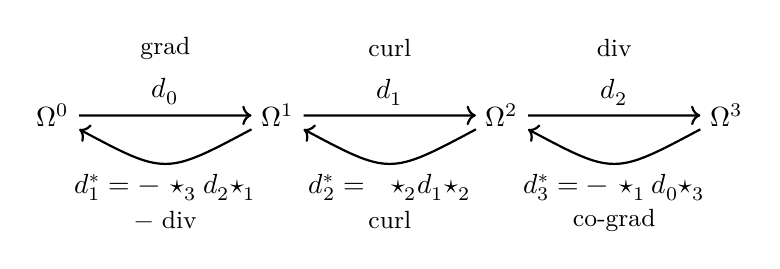
\begin{tikzpicture}[scale=0.95]
% nodes (spaces)
\node (O0) at (0,2.0) {$\Omega^0$};
\node (O1) at (3.0,2.0) {$\Omega^1$};
\node (O2) at (6.0,2.0) {$\Omega^2$};
\node (O3) at (9.0,2.0) {$\Omega^3$};

% forward d arrows
\draw[->,thick] (O0) -- node[above] {$d_0$} (O1);
\draw[->,thick] (O1) -- node[above] {$d_1$} (O2);
\draw[->,thick] (O2) -- node[above] {$d_2$} (O3);

% backward d* arrows
\draw[->,thick] (O3) .. controls (7.5,1.2) .. node[below] {$d_3^*=-\,\star_1 d_0 \star_3$} (O2);
\draw[->,thick] (O2) .. controls (4.5,1.2) .. node[below] {$d_2^*=\ \ \star_2 d_1 \star_2$} (O1);
\draw[->,thick] (O1) .. controls (1.5,1.2) .. node[below] {$d_1^*=-\,\star_3 d_2 \star_1$} (O0);

% annotations
\node at (1.5,2.9) {\small grad};
\node at (4.5,2.9) {\small curl};
\node at (7.5,2.9) {\small div};

\node at (1.5,0.6) {\small $-\,\operatorname{div}$};
\node at (4.5,0.6) {\small curl};
\node at (7.5,0.6) {\small co\mbox{-}grad};
\end{tikzpicture}
\end{center}

\end{frame}


\begin{frame}{Domains/Codomains}
    \begin{block}{ $D=3$}
\begin{align*}
&f\in\Omega^0 \xrightarrow{d_0} df\in\Omega^1,\\
&\omega\in\Omega^1 \xrightarrow{d_1} d\omega\in\Omega^2,\\
&\eta\in\Omega^2 \xrightarrow{d_2} d\eta\in\Omega^3,\\
&\alpha\in\Omega^1 \xrightarrow{d_1^*} d_1^*\alpha\in\Omega^0,\\
&\beta\in\Omega^2 \xrightarrow{d_2^*} d_2^*\beta\in\Omega^1,\\
&\gamma\in\Omega^3 \xrightarrow{d_3^*} d_3^*\gamma\in\Omega^2.
\end{align*}
\end{block}
\end{frame}

\begin{frame}{Setup and Field Quantities}
\vspace{-0.2cm}
\begin{block}{Geometric–Physical Setting}
Let $D\in\mathbb{N}$. Let $(M,g)$ be a compact, oriented $D$–dimensional Riemannian manifold with nonempty boundary $\partial M$ (spatial domain).
Let $t_0\in\mathbb{R}$ and $I=[t_0,\infty)$ (time interval).
We study the transport of an extensive quantity (mass, charge, energy, \dots) in $M$ over $I$.
\end{block}
\vspace{-0.2cm}
\begin{block}{Differential–Form Fields (time–dependent)}
%\vspace{-0.8cm}
Amount (density $D$–form): $Q\in C^\infty\!\big(I,\Omega^D M\big)$ so that $\int_V Q(t)$ is the amount in $V\subseteq M$.\\

Flow rate (flux $(D\!-\!1)$–form): $q\in C^\infty\!\big(I,\Omega^{D-1} M\big)$, so that $\int_S q(t)$ is net flow through $S^{D-1}$.\\

Internal production (source $D$–form): $f\in C^\infty\!\big(I,\Omega^D M\big),$ so that $\int_V f(t)$ is total production in $V.$
\end{block}
\end{frame}

% ------------------------------------------------------------

\begin{frame}{Flux Across an Internal Interface}
\vspace{-0.2cm}
\begin{center}
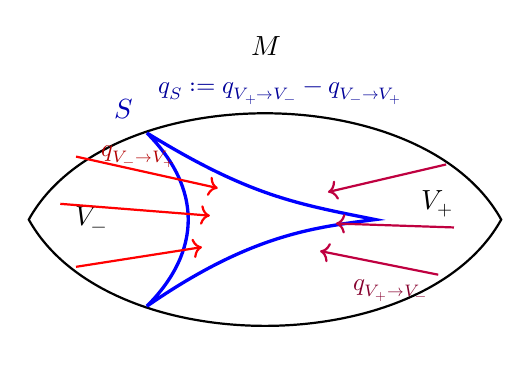
\begin{tikzpicture}[scale=1.0]
% Outer domain M (ellipsoid-like)
\draw[thick]
  (-3,0) .. controls (-2,1.8) and (2,1.8) .. (3,0)
  .. controls (2,-1.8) and (-2,-1.8) .. (-3,0) -- cycle;
\node at (0,2.2) {$M$};

% Internal interface S
\draw[very thick, blue]
  (-1.5,1.1) .. controls (-0.8,0.4) and (-0.8,-0.4) .. (-1.5,-1.1)
  .. controls (-0.2,-0.2) and (0.6,-0.1) .. (1.4,0)
  .. controls (0.4,0.2) and (-0.2,0.3) .. (-1.5,1.1);
\node[blue!70!black] at (-1.8,1.4) {$S$};

% Left region V_-
\node at (-2.2,0) {$V_{-}$};
% Right region V_+
\node at (2.2,0.2) {$V_{+}$};

% Flux arrows (left-to-right)
\draw[->,red,thick] (-2.4,0.8) -- (-0.6,0.4);
\draw[->,red,thick] (-2.6,0.2) -- (-0.7,0.05);
\draw[->,red,thick] (-2.4,-0.6) -- (-0.8,-0.35);
\node[red!70!black] at (-1.6,0.8) {\small $q_{V_{-}\to V_{+}}$};

% Flux arrows (right-to-left)
\draw[->,purple,thick] (2.3,0.7) -- (0.8,0.35);
\draw[->,purple,thick] (2.4,-0.1) -- (0.9,-0.05);
\draw[->,purple,thick] (2.2,-0.7) -- (0.7,-0.4);
\node[purple!70!black] at (1.6,-0.9) {\small $q_{V_{+}\to V_{-}}$};

% Net flux label
\node[blue!60!black] at (0.2,1.6) {\small $q_S := q_{V_{+}\to V_{-}} - q_{V_{-}\to V_{+}}$};
\end{tikzpicture}
\end{center}
\vspace{-0.6cm}
\begin{block}{Time–Integrated Net Flux Through $S$}
For $[t_1,t_2]\subset I$,
\begin{align*}
\text{Net flux on }[t_1,t_2]:\qquad
\int_{t_1}^{t_2}\!\Big(\int_S q(t)\Big)\,dt.
\end{align*}
\end{block}
\end{frame}

% ------------------------------------------------------------

\begin{frame}{Continuity Law: Integral and Differential Forms}
\vspace{-0.3cm}
\begin{block}{Integral Balance on Any Subregion $V\subseteq M$}
For $[t_1,t_2]\subset I$,
\begin{align*}
\underbrace{\int_V Q(t_2) - \int_V Q(t_1)}_{\text{amount change in }V}
&=\underbrace{\int_{t_1}^{t_2}\!\!\Big(\int_V f(t)\Big)\,dt}_{\text{internal production}}
\;-\;
\underbrace{\int_{t_1}^{t_2}\!\!\Big(\int_{\partial V} q(t)\Big)\,dt}_{\text{total outflow through }\partial V}.
\end{align*}
Using Stokes–Cartan on $\partial V$,
\begin{align*}
\int_{\partial V} q(t)=\int_V d_{D-1}q(t).
\end{align*}
\end{block}
\end{frame}


\begin{frame}{Continuity Law}
\vspace{-0.3cm}
\begin{block}{Integral Balance on Any Subregion $V\subseteq M$}
Assuming smoothness, differentiate under the integral in time:
\begin{align*}
\int_V \frac{\partial Q}{\partial t}(t)\,=\,\int_V \big(f(t)-d_{D-1}q(t)\big).
\end{align*}
\end{block}

\begin{block}{Localization (``Dropping the Integrals'')}
Because the equality holds for \emph{all} subregions $V$ and for all $t$,
the integrands must agree pointwise:
\begin{align*}
\boxed{\;\frac{\partial Q}{\partial t}\;=\;f\;-\;d_{D-1}q\;}\qquad\text{on }M\times I.
\end{align*}
This is the differential–form version of the continuity law.
\end{block}
\end{frame}

% ------------------------------------------------------------

\begin{frame}{Boundary Sign Convention and Stokes on Moving Slices}
\begin{block}{Orientation and Signs}
With the outward orientation on $\partial V$,
\begin{align*}
\int_{\partial V} q=\int_V d_{D-1}q
\quad\Longrightarrow\quad
\text{outflow (through }\partial V)\;=\;\int_V d_{D-1}q.
\end{align*}
Thus,
\begin{align*}
\frac{\partial Q}{\partial t}=f-d_{D-1}q
\end{align*}
encodes ``time rate of change = production $-$ outflow''.
\end{block}
\end{frame}


\begin{frame}{Visualization}
\begin{block}{}
\begin{center}
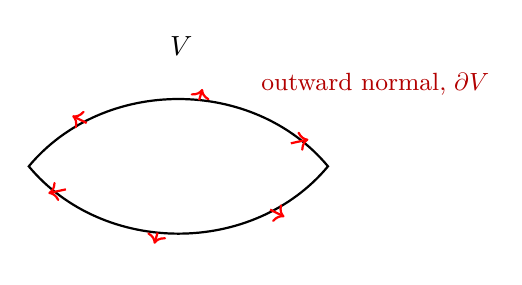
\begin{tikzpicture}[scale=0.95]
% Region V
\draw[thick]
  (-2,0) .. controls (-1,1.2) and (1,1.2) .. (2,0)
  .. controls (1,-1.2) and (-1,-1.2) .. (-2,0) -- cycle;
\node at (0,1.6) {$V$};

% Boundary with outward arrows
\foreach \a in {20,80,140,200,260,320}{
  \draw[->,red,thick]
    ({1.6*cos(\a)},{0.9*sin(\a)})
    -- ({1.85*cos(\a)},{1.05*sin(\a)});
}
\node[red!70!black] at (2.6,1.1) {\small outward normal, $\partial V$};
\end{tikzpicture}
\end{center}
\end{block}


\end{frame}
% ------------------------------------------------------------

\begin{frame}{Correspondence with Vector Calculus}
\vspace{-0.3cm}
\begin{block}{A Common Identification}
In $D=3$, write $Q=\tilde{\rho}\,dV$ (amount density $\tilde{\rho}$ times $3$–volume form),
and represent a vector flux field $\tilde{F}$ via the flux $2$–form $q=\iota_{\tilde{F}}\mathrm{vol}$.
Then
\begin{align*}
&\frac{\partial Q}{\partial t}=f-d_2 q
\quad\Longleftrightarrow\quad
\frac{\partial \tilde{\rho}}{\partial t}\,dV
= \tilde{f}\,dV - (\nabla\cdot \tilde{F})\,dV
\\
&\Longleftrightarrow\quad
\boxed{\;\frac{\partial \tilde{\rho}}{\partial t}=\tilde{f}-\nabla\cdot \tilde{F}\;}.
\end{align*}
\end{block}
\vspace{-0.3cm}
\begin{center}
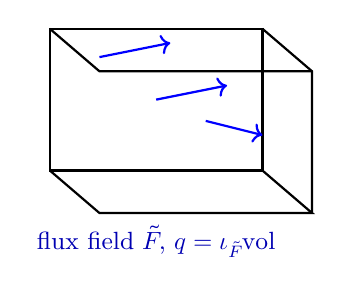
\begin{tikzpicture}[scale=0.9]
% 3D-ish box
\draw[thick] (0,0) rectangle (3,2);
\draw[thick] (0,0) -- (0.7,-0.6) -- (3.7,-0.6) -- (3,0);
\draw[thick] (3,2) -- (3.7,1.4) -- (3.7,-0.6);
\draw[thick] (0,2) -- (0.7,1.4) -- (3.7,1.4);

% Vector field arrows
\draw[->,blue,thick] (1.5,1.0) -- (2.5,1.2);
\draw[->,blue,thick] (0.7,1.6) -- (1.7,1.8);
\draw[->,blue,thick] (2.2,0.7) -- (3.0,0.5);
\node[blue!70!black] at (1.5,-1.0) {\small flux field $\tilde{F}$, $q=\iota_{\tilde{F}}\mathrm{vol}$};
\end{tikzpicture}
\end{center}
\end{frame}

% ------------------------------------------------------------


\begin{frame}{Neumann Boundary and Prescribed Flux}
\begin{block}{Boundary Portion and Data}
Let $\Gamma_N\subseteq\partial M$ be a $(D\!-\!1)$–dimensional smooth submanifold (Neumann boundary).
A \emph{prescribed} flux (i.e.\ \emph{given as boundary input}) is a $(D\!-\!1)$–form
\begin{align*}
g_N\in C^\infty\!\big(I,\Omega^{D-1}\Gamma_N\big)\quad\text{with physical unit }[X\,T^{-1}],
\end{align*}
interpreted so that $\int_S g_N(t)$ equals the net amount per unit time crossing $S\subset\Gamma_N$ at time $t$.
\end{block}
\vspace{-0.3cm}
\begin{block}{Neumann Boundary Condition (NBC)}
The total flux $q\in C^\infty\!\big(I,\Omega^{D-1}M\big)$ satisfies
\begin{align*}
\operatorname{tr}_{\Gamma_N} q \;=\; g_N \qquad \text{on } \Gamma_N\times I.
\end{align*}
\end{block}

\end{frame}

\begin{frame}{Neumann Boundary and Prescribed Flux}
\begin{block}{Boundary Portion and Data}
\begin{center}
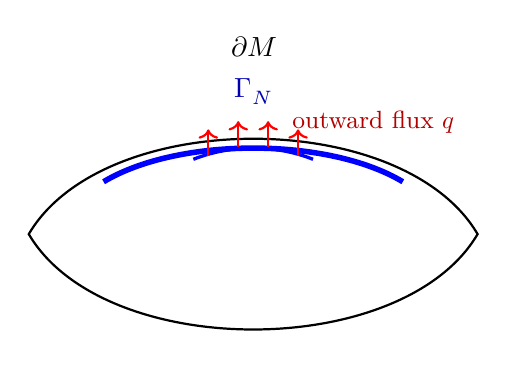
\begin{tikzpicture}[scale=0.95]
% Outer boundary
\draw[thick]
  (-3,0) .. controls (-2,1.7) and (2,1.7) .. (3,0)
  .. controls (2,-1.7) and (-2,-1.7) .. (-3,0) -- cycle;
\node at (0,2.5) {$\partial M$};

% Mark Gamma_N arc (top)
\draw[line width=2pt, blue]
  (-2.0,0.7) .. controls (-1.0,1.3) and (1.0,1.3) .. (2.0,0.7);
\node[blue!70!black] at (0, 1.9) {$\Gamma_N$};

% A boundary segment S subset Gamma_N with outward normals
\draw[very thick, blue] (-0.8,1.0) .. controls (-0.3,1.2) and (0.3,1.2) .. (0.8,1.0);
\foreach \x/\y in {-0.6/1.05,-0.2/1.16,0.2/1.16,0.6/1.05}{
  \draw[->,red,thick] (\x,\y) -- (\x,\y+0.35);
}
\node[red!70!black] at (1.6,1.50) {\small outward flux $q$};
\end{tikzpicture}
\end{center}
\end{block}
\end{frame}

% ---------------------------------------------------------

\begin{frame}{Potential, Diffusion, and Advection}
\vspace{-0.3cm}
\begin{block}{Potential and Total Flux Split}
Let $u\in C^\infty\!\big(I,\Omega^{0}M\big)$ be the \emph{potential} (units $[Y]$), e.g.\ temperature, concentration, pressure, or electric potential.
Split the total flux as
\begin{align*}
q \;=\; q_D \;+\; q_A ,
\end{align*}
where $q_D$ is the \emph{diffusive} part and $q_A$ is the \emph{advective} part.
\end{block}

\vspace{-0.3cm}
\begin{block}{Diffusive (constitutive) law — isotropic \& anisotropic}
With $du\in\Omega^{1}M$ and Hodge star $\star:\Omega^{1}\!\to\!\Omega^{D-1}$,
\begin{align*}
\text{(isotropic)} \quad & q_D \;=\; -\,\kappa\,\star(du),
\quad \kappa\in C^\infty(M),\ \kappa>0;\\
\text{(anisotropic)} \quad & q_D \;=\; -\,\star\!\big(\,\widetilde{\kappa}(du)\big),
\quad \widetilde{\kappa}:\Omega^{1}M\to\Omega^{1}M\\
&\text{(SPD $(1,1)$–tensor)}.
\end{align*}
\end{block}
\end{frame}

\begin{frame}{Potential, Diffusion, and Advection}
\begin{block}{Diffusive (constitutive) law — isotropic \& anisotropic}

Equivalently, define $\kappa:\Omega^{D-1}\!M\to\Omega^{D-1}\!M$ by the identity
\begin{align*}
\boxed{\;\star_{D-1}\circ \widetilde{\kappa} \;=\; \kappa \circ \star_{1}\;}
\qquad\Rightarrow\qquad
q_D \;=\; -\,\kappa\,\star(du).
\end{align*}
\begin{center}
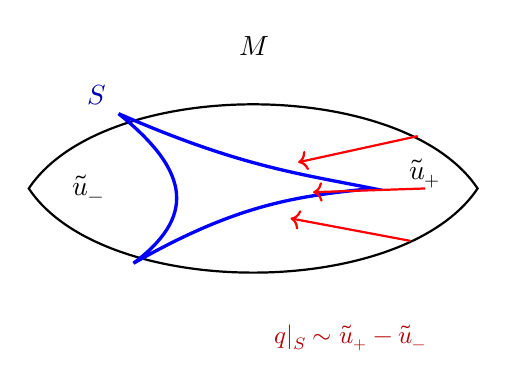
\begin{tikzpicture}[scale=0.95]
% Domain M
\draw[thick]
  (-3,0) .. controls (-2,1.5) and (2,1.5) .. (3,0)
  .. controls (2,-1.5) and (-2,-1.5) .. (-3,0) -- cycle;
\node at (0,1.9) {$M$};

% Internal interface S
\draw[very thick, blue]
  (-1.8,1.0) .. controls (-0.8,0.2) and (-0.8,-0.4) .. (-1.6,-1.0)
  .. controls (-0.2,-0.2) and (0.6,-0.1) .. (1.6,0.0)
  .. controls (0.6,0.2) and (-0.2,0.3) .. (-1.8,1.0);
\node[blue!70!black] at (-2.1,1.25) {$S$};

% Labels u_- and u_+
\node at (-2.2,0) {$\widetilde{u}_{-}$};
\node at (2.3,0.2) {$\widetilde{u}_{+}$};

% Arrows indicating flow right->left (u_+ > u_-)
\draw[->,red,thick] (2.2,0.7) -- (0.6,0.35);
\draw[->,red,thick] (2.3,0.0) -- (0.8,-0.05);
\draw[->,red,thick] (2.1,-0.7) -- (0.5,-0.4);
\node[red!70!black] at (1.3, -2.0) {\small $q|_S \sim \widetilde{u}_{+}-\widetilde{u}_{-}$};
\end{tikzpicture}
\end{center}
\end{block}


\end{frame}


\begin{frame}{Advection}
\begin{block}{Advective Flux via Volume Flux Form}
Let $\widetilde{v}$ be a velocity vector field; its \emph{volume flux form} is
\begin{align*}
v \;:=\; \iota_{\widetilde{v}}\,\mathrm{vol}\;\in\;\Omega^{D-1}M
\qquad(\text{units }[L^D T^{-1}]).
\end{align*}
If $Q\in\Omega^{D}M$ is the amount $D$–form, then
\begin{align*}
\boxed{\;q_A \;=\; (\star Q)\,v\;}\qquad
\left(\text{scalar density }\star Q\ \times\ \text{volume flux form }v\right).
\end{align*}
\end{block}
\end{frame}

\begin{frame}{Capacity}
\begin{block}{Volumetric Capacity}
Relate amount and potential by a capacity coefficient:
\begin{align*}
&\widetilde{\pi}:\Omega^{0}M\to\Omega^{0}M,\qquad
Q \;=\; \star\big(\,\widetilde{\pi}\,u\,\big).\\
&\text{Equivalently, }\ \exists\,\pi:\Omega^{D}\!M\to\Omega^{D}\!M\ \text{with}\
\boxed{\;\pi\circ \star_{0} \;=\; \star_{0}\circ \widetilde{\pi}\;},\\
&
\Rightarrow\quad Q=\pi(\star u).
\end{align*}
Hence
\begin{align*}
\frac{\partial Q}{\partial t}
\;=\; \pi\!\left(\star\,\frac{\partial u}{\partial t}\right)
\;=\; \star\!\left(\widetilde{\pi}\,\frac{\partial u}{\partial t}\right).
\end{align*}
\end{block}
\end{frame}

\begin{frame}{Boundary Partition and Data}
\begin{block}{Dirichlet vs.\ Neumann}
Let $\Gamma_D,\Gamma_N\subseteq\partial M$ be relatively open, disjoint, with
\begin{align*}
\Gamma_D\cup\Gamma_N=\partial M,
\qquad \dim(\Gamma_D\cap\Gamma_N)\le D-2.
\end{align*}
Dirichlet boundary condition (DBC):
\begin{align*}
\operatorname{tr}_{\Gamma_D} u \;=\; u_D,\qquad u_D\in C^\infty(I,\Omega^0 \Gamma_D).
\end{align*}
Neumann boundary condition (NBC):
\begin{align*}
\operatorname{tr}_{\Gamma_N} q \;=\; g_N,\qquad g_N\in C^\infty(I,\Omega^{D-1} \Gamma_N).
\end{align*}
\end{block}
\end{frame}

\begin{frame}{Visualization}
    \begin{block}{}
        \begin{center}
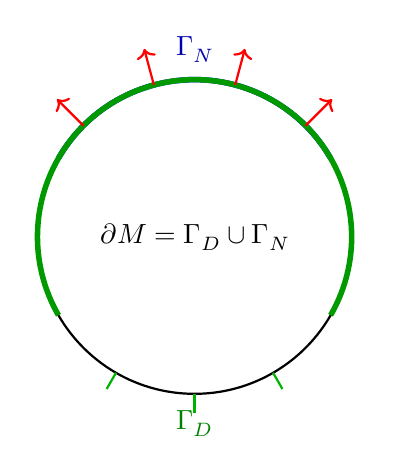
\begin{tikzpicture}[scale=0.95]
% circle boundary
\draw[thick] (0,0) circle (2.1);
% upper arc Gamma_N
\draw[line width=2pt, blue] (150:2.1) arc (150:30:2.1);
\node[blue!70!black] at (0,2.5) {$\Gamma_N$};
% lower arc Gamma_D
\draw[line width=2pt, green!60!black] (-30:2.1) arc (-30:210:2.1);
\node[green!50!black] at (0,-2.5) {$\Gamma_D$};

% Sample outward normal arrows on Gamma_N
\foreach \a in {45,75,105,135}{
  \draw[->,red,thick] (\a:2.1) -- (\a:2.6);
}
% Sample markers on Gamma_D
\foreach \a in {240,270,300}{
  \draw[green!70!black,thick] (\a:2.1) -- (\a:2.35);
}
\node at (0,0) {$\partial M=\Gamma_D\cup\Gamma_N$};
\end{tikzpicture}
\end{center}
    \end{block}
\end{frame}

% ---------------------------------------------------------

\begin{frame}{Governing Equations (Summary)}
\begin{block}{Bulk Law (Continuity)}
\begin{align*}
\frac{\partial Q}{\partial t} \;=\; f \;-\; d_{D-1} q
\qquad\text{in }M\times I.
\end{align*}
\end{block}

\begin{block}{Constitutive Relations}
\begin{align*}
&\text{Capacity:}\qquad Q \;=\; \star\!\left(\widetilde{\pi}\,u\right) \;=\; \pi(\star u),
\quad \pi\circ \star_{0}=\star_{0}\circ \widetilde{\pi}.\\[2pt]
&\text{Diffusion:}\qquad q_D \;=\; -\,\star\!\big(\,\widetilde{\kappa}(du)\big)
\;=\; -\,\kappa\,\star(du),
\quad \star_{D-1}\circ \widetilde{\kappa}=\kappa\circ \star_1.\\[2pt]
&\text{Advection:}\qquad q_A \;=\; (\star Q)\,v,
\quad v=\iota_{\widetilde{v}}\mathrm{vol}\in\Omega^{D-1}M.
\end{align*}
\end{block}
\end{frame}


\begin{frame}{Governing Equations (Summary)}
\begin{block}{Boundary Conditions and Unknowns}
\begin{align*}
&\text{Unknowns: } u\in C^\infty(I,\Omega^{0}M),\quad
Q\in C^\infty(I,\Omega^{D}M),\\
&q\in C^\infty(I,\Omega^{D-1}M).\\
&\text{Dirichlet on }\Gamma_D:\quad \operatorname{tr}_{\Gamma_D} u = u_D.\\
&\text{Neumann on }\Gamma_N:\quad \operatorname{tr}_{\Gamma_N} q = g_N.\\
&\text{Total flux:}\quad q = q_D + q_A.
\end{align*}
\end{block}
\end{frame}

% (from $Q,q$ expressed via $u$)
\begin{frame}{Primal Strong Model}
%\vspace{-0.3cm}
\begin{block}{Continuity and Constitutive Content (recall)}
\vspace{-0.5cm}
\begin{align*}
&\text{Continuity:}\qquad \frac{\partial Q}{\partial t}\;=\; f\;-\; d_{D-1} q,\\[2pt]
&\text{Amount--potential link (capacity):}\qquad Q \;=\; \star\!\big(\widetilde{\pi}\,u\big)
\\
&\big(\text{equivalently } \widetilde{\pi}\,u=\star_D Q\big),\\[2pt]
&\text{Flux split:}\qquad q \;=\; q_D + q_A,\\
&\hspace{1.7cm}\text{Diffusion (anisotropic): } q_D=-\,\star\!\big(\widetilde{\kappa}\,du\big)
\\
&\big(\text{isotropic: }q_D=-\,\kappa\,\star du\big),\\
&\hspace{1.7cm}\text{Advection: } q_A=(\star Q)\,v,\quad v=\iota_{\widetilde{v}}\mathrm{vol}\in\Omega^{D-1}M.
\end{align*}
\end{block}

\end{frame}


\begin{frame}{Primal Strong Model}

\begin{block}{Substitute $Q,q$ in terms of $u$}
\begin{align*}
\frac{\partial}{\partial t}\Big(\star\!\big(\widetilde{\pi}\,u\big)\Big)
&= f - d_{D-1}\!\Big( -\,\star(\widetilde{\kappa}\,du) \;+\; (\star Q)\,v\Big)\\[2pt]
&= f \;+\; d_{D-1}\star(\widetilde{\kappa}\,du) \;-\; d_{D-1}\!\big((\star Q)\,v\big)\\[2pt]
&= f \;+\; d_{D-1}\star(\widetilde{\kappa}\,du) \;-\; d_{D-1}\!\Big((\star\star(\widetilde{\pi}u))\,v\Big),
\end{align*}
where in the last line we used $Q=\star(\widetilde{\pi}u)$.
\end{block}
\end{frame}

\begin{frame}{Primal Strong Model}
\begin{block}{Primal strong equation for $u$}
\begin{align*}
\boxed{\;
\frac{\partial}{\partial t}\Big(\star(\widetilde{\pi}u)\Big)
\;-\; d_{D-1}\star(\widetilde{\kappa}\,du)
\;+\; d_{D-1}\!\Big((\star\star(\widetilde{\pi}u))\,v\Big)
\;=\; f
\;}
\end{align*}
In isotropic diffusion ($\widetilde{\kappa}=\kappa\,\operatorname{id}$), the second term is $d_{D-1}(\kappa\,\star du)$.
\end{block}
\end{frame}

\begin{frame}{Equivalent Form Using $\;\widetilde{\pi}u=\star_D Q$}
\vspace{-0.3cm}
\begin{block}{Express everything through $Q$ and then back to $u$}
\vspace{-0.9cm}
\begin{align*}
\widetilde{\pi}u=\star_D Q
&\quad\Longleftrightarrow\quad
\star(\widetilde{\pi}u)=\star\star_D Q
\;\;=\;\sigma_D\,Q,
\end{align*}
where $\sigma_D=\pm 1$ depends on the metric signature and $D$ (in Euclidean $D$–RM, $\sigma_D=+1$). Hence
\vspace{-0.4cm}
\begin{align*}
\frac{\partial}{\partial t}\Big(\star(\widetilde{\pi}u)\Big)
= \sigma_D\,\frac{\partial Q}{\partial t}.
\end{align*}
Using the continuity equation $\frac{\partial Q}{\partial t}=f-d_{D-1}q$ and $q=-\star(\widetilde{\kappa}du)+(\star Q)v$, we get
\vspace{-0.4cm}
\begin{align*}
\sigma_D\,\frac{\partial Q}{\partial t}
&= f - d_{D-1}\!\Big(-\star(\widetilde{\kappa}du)+(\star Q)v\Big)\\
&= f + d_{D-1}\star(\widetilde{\kappa}du) - d_{D-1}\!\big((\star Q)v\big).
\end{align*}
Replacing $Q$ by $\star(\widetilde{\pi}u)$ recovers the primal equation in $u$ from the previous slide.
\end{block}
\end{frame}

% ---------------------------------------------------------

\begin{frame}{Manufactured Steady Problem}

\begin{block}{Steady assumptions and model}
Let $\frac{\partial u}{\partial t}=0$, hence $\frac{\partial Q}{\partial t}=0$, and $v=0$.
The continuity law reduces to
\begin{align*}
0 \;=\; f - d_{D-1}q \quad\Longrightarrow\quad f \;=\; d_{D-1}q.
\end{align*}
With pure diffusion $q=q_D=-\,\kappa\,\star du$ (isotropic, constant $\kappa>0$),
\begin{align*}
f \;=\; d_{D-1}\!\big(-\,\kappa\,\star du\big) \;=\; -\,\kappa\, d_{D-1}\!\big(\star du\big).
\end{align*}
\end{block}
\end{frame}

\begin{frame}{Manufactured Steady Problem}
\vspace{-0.3cm}
\begin{block}{Choose $M=[0,1]^3\subset\mathbb{R}^3$, standard Euclidean metric}
Let $u(x,y,z)=x^2+y^2+z^2$ and $\kappa=2$ (constant).
\vspace{-0.4cm}
\begin{align*}
du &= 2x\,dx + 2y\,dy + 2z\,dz,\\[2pt]
\star dx &= dy\wedge dz,\quad \star dy = dz\wedge dx,\quad \star dz = dx\wedge dy,\\[2pt]
\star du &= 2x\,dy\wedge dz \;+\; 2y\,dz\wedge dx \;+\; 2z\,dx\wedge dy,\\[2pt]
q \;=\; -\,\kappa\,\star du
&= -\,2\Big(2x\,dy\wedge dz + 2y\,dz\wedge dx + 2z\,dx\wedge dy\Big)\\
&= -\,4x\,dy\wedge dz \;-\; 4y\,dz\wedge dx \;-\; 4z\,dx\wedge dy.
\end{align*}
Finally,
\vspace{-0.5cm}
\begin{align*}
f &=\; d q \;=\; -\,\kappa\, d(\star du)
= -\,2\,\big(\Delta u\big)\,dx\wedge dy\wedge dz
= -\,2\cdot 6\,dx\wedge dy\wedge dz\\
&= -\,12\,dx\wedge dy\wedge dz.
\end{align*}
\vspace{-0.1cm}
Thus the manufactured source is the constant $3$–form $f=-12\,dx\wedge dy\wedge dz$ on $M$.
\end{block}
\end{frame}

\begin{frame}{Flux Sketch (steady diffusion in a cube)}
\begin{center}
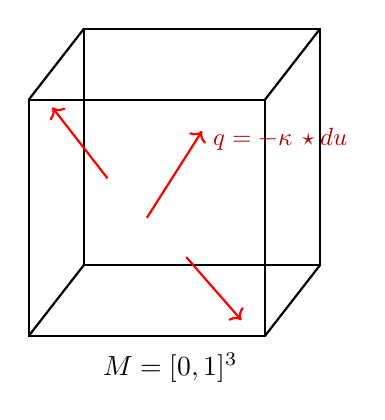
\begin{tikzpicture}[scale=1.0]
% A cube outline
\draw[thick] (0,0) rectangle (3,3);
\draw[thick] (0.7,0.9) -- (3.7,0.9) -- (3.7,3.9) -- (0.7,3.9) -- cycle;
\draw[thick] (3,3) -- (3.7,3.9);
\draw[thick] (0,3) -- (0.7,3.9);
\draw[thick] (3,0) -- (3.7,0.9);
\draw[thick] (0,0) -- (0.7,0.9);
\node at (1.8,-0.4) {$M=[0,1]^3$};

% A few indicative flux arrows (pointing outward where u increases)
\draw[->,red,thick] (1.5,1.5) -- (2.2,2.6);
\draw[->,red,thick] (1.0,2.0) -- (0.3,2.9);
\draw[->,red,thick] (2.0,1.0) -- (2.7,0.2);
\node[red!70!black] at (3.2,2.5) {\small $q=-\kappa\,\star du$};
\end{tikzpicture}
\end{center}
\end{frame}

% ---------------------------------------------------------



\begin{frame}{Summary}
\begin{block}{Main Concepts}
\begin{itemize}
\item $\mu(M)=\int_M \mathrm{vol}_{(M,g)}$ gives measure (length/area/volume) of $(M,g)$.
\item $\langle \omega,\eta\rangle_p=\int_M g_p^*(\omega,\eta)\mathrm{vol}_{(M,g)}$ defines inner product on $\Omega^p(M)$.
\item Codifferential $d^*$ is the adjoint of $d$:
\begin{align*}
\langle d_p^*\omega,\eta\rangle_{p-1}=\langle \omega,d_{p-1}\eta\rangle_p.
\end{align*}
\item Relationship with Hodge star:
\begin{align*}
d_{D-p}^*\circ\star_p=(-1)^{p+1}\star_{p+1}\circ d_p.
\end{align*}
\item For $D=3$: $(d_0,d_1,d_2)$ correspond to $(\nabla,\nabla\times,\nabla\cdot)$ and $(d_1^*,d_2^*)$ to their adjoints.
\end{itemize}
\end{block}
\end{frame}


\begin{frame}{Summary}
\begin{block}{Main Concepts}
\begin{itemize}
\item Neumann data prescribes the \emph{flux} $(D\!-\!1)$–form on $\Gamma_N$, Dirichlet data prescribes the \emph{potential} on $\Gamma_D$.
\item Diffusion: $q_D=-\star(\widetilde{\kappa}\,du)$ (or $-\kappa\,\star du$); Advection: $q_A=(\star Q)\,v$ with $v=\iota_{\widetilde{v}}\mathrm{vol}$.
\item Capacity links amount and potential: $Q=\star(\widetilde{\pi}u)$.
\item Continuity in forms: $\displaystyle \frac{\partial Q}{\partial t}=f-d_{D-1}q$, closed by the constitutive laws and boundary conditions.
\end{itemize}
\end{block}
\end{frame}

\begin{frame}{Summary}
\begin{block}{Main Concepts}
\begin{itemize}
\item Amount $Q(t)\in\Omega^D M$, flux $q(t)\in\Omega^{D-1} M$, production $f(t)\in\Omega^D M$ model transport on $(M,g)$.
\item Integral balance on any $V\subseteq M$ and Stokes–Cartan yield the local continuity law
\begin{align*}
\frac{\partial Q}{\partial t}=f-d_{D-1}q.
\end{align*}
\item In $D=3$, with $Q=\tilde{\rho}\,dV$ and $q=\iota_{\tilde{F}}\mathrm{vol}$, this becomes
\begin{align*}
\frac{\partial \tilde{\rho}}{\partial t}=\tilde{f}-\nabla\cdot \tilde{F}.
\end{align*}
\end{itemize}
\end{block}
\end{frame}

\begin{frame}{Summary}
\begin{block}{Main Concepts}
\begin{itemize}
\item Primal strong model (exterior–calculus form):
\begin{align*}
\frac{\partial}{\partial t}\big(\star(\widetilde{\pi}u)\big)
- d_{D-1}\star(\widetilde{\kappa}du)
+ d_{D-1}\!\big((\star\star(\widetilde{\pi}u))v\big) \;=\; f.
\end{align*}
\item Steady, no advection: $f=dq=-\kappa\,d(\star du)$; in $\mathbb{R}^3$ this is $f=-\kappa\,\Delta u\,\mathrm{vol}$.
\item Manufactured 3D example with $u=x^2+y^2+z^2$, $\kappa=2$:
$q=-4x\,dy\wedge dz-4y\,dz\wedge dx-4z\,dx\wedge dy$, \; $f=-12\,dx\wedge dy\wedge dz$.
\end{itemize}
\end{block}
\end{frame}

\begin{frame}{Global Picture}
\vspace{-0.3cm}
\begin{center}
\begin{tikzpicture}[
    scale=0.85, % OVERALL SCALE: increase to enlarge entire diagram
    >=latex,
    % Box style: adjust inner sep, minimum width/height, font size
    box/.style={draw,rounded corners,align=center,fill=#1!10,inner sep=1pt,minimum width=0.7cm,minimum height=0.3cm,font=\tiny},
    % Label style: adjust font size
    lbl/.style={font=\tiny,inner sep=0.3pt}
]

% ==============================
% TUNING KNOBS - EDIT THESE TO ADJUST POSITIONS
% ==============================
\def\xL{-2.7}   % LEFT COLUMN x-position (move left: decrease, move right: increase)
\def\xR{1.8}    % RIGHT COLUMN x-position (spacing between columns = xR - xL)
\def\yTop{4.2}  % TOP ROW y-position (move up: increase, move down: decrease)
\def\dy{1.4}    % VERTICAL SPACING between rows (increase for more space)

% CORNER BOXES POSITIONS
\def\xLT{-5.0}  % TOP-LEFT corner x (potential u)
\def\yLT{4.5}   % TOP-LEFT corner y
\def\xLB{-5.0}  % BOTTOM-LEFT corner x (flow rate q)
\def\yLB{-0.5}  % BOTTOM-LEFT corner y
\def\xRT{7.5}   % TOP-RIGHT corner x (aux 1-form)
\def\yRT{4.5}   % TOP-RIGHT corner y
\def\xRB{7.5}   % BOTTOM-RIGHT corner x (amount Q)
\def\yRB{-0.5}  % BOTTOM-RIGHT corner y

% ==============================
% LEFT COLUMN: Ω^p (p=0 to D)
% ==============================
% Each node: adjust minimum width/height in box style, or add locally
\node[box=white] (L0)  at (\xL,\yTop-0*\dy) {$\Omega^{0}$};
\node[box=white] (L1)  at (\xL,\yTop-1*\dy) {$\Omega^{1}$};

\node[lbl]      (Ld1) at (\xL, \yTop-2*\dy - 0.2) {$\vdots$}; % Adjust yshift (0.2) to move dots
\node[box=white] (LDm) at (\xL,\yTop-3*\dy) {$\Omega^{D-1}$};
\node[box=white] (LD)  at (\xL,\yTop-4*\dy) {$\Omega^{D}$};

% UPWARD d_p ARROWS (exterior derivative) – slightly shifted left and shortened
\draw[->,shorten >=1pt, shorten <=1pt] ([xshift=-0.10cm]L0.west) -- node[lbl,sloped,above] {$d_0$} ([xshift=-0.10cm]L1.west);

% \draw[->,shorten >=1pt, shorten <=1pt] ([xshift=-0.10cm]L1.west) -- node[lbl,sloped,above,yshift=0.5pt] {$d_1$} +([xshift = -0.10cm]0,-0.95) coordinate (tmpd);

\draw[dashed] ([xshift=-0.10cm]L1.west) -- ++(0,-0.65); % Dashed middle section

\draw[->,shorten >=1pt,shorten <=1pt] ([xshift=-0.10cm]LDm.west) -- node[lbl,sloped,above] {$d_{D-1}$} ([xshift=-0.10cm]LD.west);

% To fine-tune:
% - adjust xshift (currently -0.10cm) → move arrows further left or right
% - adjust shorten >= / <= (currently 1pt) → shorten or lengthen arrow tips
% DOWNWARD d_p^* ARROWS (codifferential)
\draw[->] (L1) -- node[lbl,sloped,above] {$d_1^{*}$} (L0);
\draw[dashed,->] ($(L1)+(0,-0.65)$) -- node[lbl,left] {$\cdots$} ($(LDm)+(0,0.65)$);
\draw[->] (LD) -- node[lbl,sloped,above] {$d_{D}^{*}$} (LDm);


% ==============================
% RIGHT COLUMN: Ω^{D-p} (mirrored by Hodge star)
% ==============================
\node[box=white] (R0)  at (\xR,\yTop-0*\dy) {$\Omega^{D}$};
\node[box=white] (R1)  at (\xR,\yTop-1*\dy) {$\Omega^{D-1}$};
\node[lbl]      (Rd1) at (\xR,\yTop-2*\dy+0.2) {$\vdots$};
\node[box=white] (RDm) at (\xR,\yTop-3*\dy) {$\Omega^{1}$};
\node[box=white] (RD)  at (\xR,\yTop-4*\dy) {$\Omega^{0}$};


% OPTIONAL: Faint d operators on right column – shifted slightly left
\draw[<-,gray!60,shorten >=1pt,shorten <=1pt] ([xshift=-0.10cm]R0.west) -- node[lbl,sloped,above] {$d_{D-1}$} ([xshift=-0.10cm]R1.west);
\draw[dashed,gray!60] ([xshift=-0.10cm]R1.west) -- ++(0,-0.65);
\draw[<-,gray!60,shorten >=1pt,shorten <=1pt] ([xshift=-0.10cm]RDm.west) -- node[lbl,sloped,above] {$d_{0}$} ([xshift=-0.10cm]RD.west);

% OPTIONAL: Faint d^* operators on right column – shifted slightly right and separated
\draw[->,gray!60,shorten >=1pt,shorten <=1pt] ([xshift=0.12cm]R0.east) -- node[lbl,sloped,below] {$d^{*}_{D}$} ([xshift=0.12cm]R1.east);
\draw[dashed,gray!60] ([xshift=0.12cm]R1.east) -- ++(0,-0.65);
\draw[->,gray!60,shorten >=1pt,shorten <=1pt] ([xshift=0.12cm]RDm.east) -- node[lbl,sloped,below] {$d^{*}_{1}$} ([xshift=0.12cm]RD.east);

% To tune:

% ==============================
% HODGE STAR PAIRS: horizontal arrows (left ↔ right)
% ==============================
\draw[<->] (L0) -- node[lbl,above] {$\star_{0}$} (R0);
\draw[<->] (L1) -- node[lbl,above] {$\star_{1}$} (R1);

\draw[dashed] ($(L1)+(0,-0.65)$) -- ($(R1)+(0,-0.65)$);

\draw[<->] (LDm) -- node[lbl,above] {$\star_{D-1}$} (RDm);
\draw[<->] (LD) -- node[lbl,above] {$\star_{D}$} (RD);

% ==============================
% FORMULA PANEL (center-right)
% Adjust: x-position, y-position, text width, font size, inner sep
% ==============================
\node[draw,rounded corners,align=left,fill=gray!10,inner sep=3pt,font=\tiny, text width=4.3cm]
    (form) at (\xR+1.8, -2.9) % Position: (x, y)
    {
    \textbf{Codifferential}:\\ $d_{D-p}^{*} =(-1)^{p+1+p(D-p)}\,\star_{p+1}\circ d_{p}\circ \star_{D-p}$\\
    \textbf{Inner product}: $g^{*}_{p}(\omega,\eta)\,\mathrm{vol} =\omega\wedge \star_{p}\eta$\\
    \textbf{Hodge involution}:\\ $\star_{D-p}\circ \star_{p}=(-1)^{p(D-p)}\,\mathrm{id}_{\Omega^{p}}$
    };

% ==============================
% CORNER BOXES: Physical variables
% Adjust: position (xLT,yLT etc.), minimum width, font size
% ==============================
\node[box=blue, minimum width=1.5cm] at (\xLT,\yLT)
    {$u\in\Omega^{0}$\\ \tiny potential};
\node[box=blue, minimum width=1.5cm] at (\xRT-2.5,\yRT)
    {$\tilde{q}\in\Omega^{1}$\\ \tiny (aux. 1-form)};
\node[box=green, minimum width=1.5cm] at (\xLB,\yLB)
    {$q\in\Omega^{D-1}$\\ \tiny flow rate};
\node[box=green, minimum width=1.5cm] at (\xRB-2.5,\yRB+2.5)
    {$Q\in\Omega^{D}$\\ \tiny amount density};

% DOTTED GUIDES from corner boxes to main columns
\draw[dotted] (\xLT+0.9,\yLT-0.25) -- (L0.west);
\draw[dotted] (\xLB+1.0,\yLB+0.25) -- (LDm.west);
\draw[dotted] (\xRT-1.9,\yRT-0.25) -- (R1.east);
\draw[dotted] (\xRB-1.9,\yRB+2.85) -- (R0.east);
\end{tikzpicture}
\end{center}
\end{frame}

\begin{frame}{Thanks}
  \cmcendframe
\end{frame}

\end{document}
